\documentclass[12pt]{article}

\usepackage{fullpage}
\usepackage{fancyhdr}
\usepackage{nopageno}
\usepackage{ifthen}
\usepackage{amsmath}
\usepackage{amssymb}
\usepackage{amsthm}
\usepackage{multicol}
\usepackage{version}
\usepackage{graphicx}
\usepackage{psfrag}
\usepackage{amssymb}
\newcommand{\R}{\mathbb{R}}
\newcommand{\N}{\mathbb{N}}

\usepackage[margin=0.75in]{geometry}
%\usepackage{nopageno}
\newcommand{\HasSolutions}{true}
\excludeversion{titlepage}
\excludeversion{filler}

%\newcommand{\HasSolutions}{false}
%\includeversion{titlepage}
%\includeversion{filler}

\ifthenelse{\equal{\HasSolutions}{true}}{\includeversion{solutiontext}}{\excludeversion{solutiontext}}

\newenvironment{solution}{\subsubsection*{Solution.}}{}

\title{Midterm 1}
\author{Math 195 Section 91}
\date{July 6, 2009}

\newcounter{problem}
\setcounter{problem}{1}

\newcounter{totalpoints}
\setcounter{totalpoints}{0}

\makeatletter
\def\inputtoc{%
    \makeatletter
    \@input{\jobname.toc}%
    \if@filesw
      \expandafter\newwrite\csname tf@toc\endcsname
      \immediate\openout \csname tf@toc\endcsname \jobname.toc\relax
    \fi
    \@nobreakfalse
    }
\makeatother

\newenvironment{problem}[1][]%
{\ifthenelse{\equal{\HasSolutions}{true}}{}{\pagebreak}%
\addtocounter{totalpoints}{#1}%
%\ifthenelse{\equal{\HasSolutions}{true}}{}{\rfoot{\fbox{\Huge\hspace{2em}/#1}}}
\ifthenelse{\equal{\HasSolutions}{true}}{\vspace{3ex}\noindent\makebox[0in]{\vspace{5ex}\hspace{-1em}\rule{1ex}{3ex}\raisebox{2ex}{\rule{2ex}{1ex}}}\vspace{-6ex}}{}%
\subsection*{Problem \arabic{problem}.%
\addtocontents{toc}{Problem \arabic{problem} \protect& \hspace{2em} \protect& /#1 \protect\\ \protect\hline}%
\ifthenelse{\equal{\HasSolutions}{true}}{}{\hfill\fbox{\Huge\hspace{2em}/#1}}
}}%
{%
\addtocounter{problem}{1}%
%\ifthenelse{\equal{\HasSolutions}{true}}{}{\vfill\fbox{\Huge\hspace{2em}/#1}}%
}%

\renewcommand{\headrulewidth}{0in}

\cfoot{}

\newcommand{\answerbox}[1]{\ifthenelse{\equal{\HasSolutions}{true}}{\fbox{#1}}{#1}}

\newcommand{\TrueChoice}{\answerbox{True} False}
\newcommand{\FalseChoice}{True \answerbox{False}}

\begin{document}

\setlength{\headheight}{30pt}

%%%%%%%%%%%%%%%%%%%%%%%%%%%%%%%%%%%%%%%%%%%%%%%%%%%%%%%%%%%%%%%%
% Cover Page
%\markboth{}{\hfill\textbf{Name:} \underline{Solution Set} \\}

\begin{titlepage}
\maketitle

\begin{center}
$$
\int \frac{1}{\mbox{cabin}} \, d\mbox{cabin} = \log \mbox{cabin} + \mbox{sea}.
$$
\end{center}
\vfill
\vfill

\noindent
\hspace{1in}
\textbf{Name: } \hrulefill
\hspace{1in}

\vfill

\begin{multicols}{2}
\begin{enumerate}
\item Write your name above.
\item Do not look inside the exam until instructed to do so.
\item You have \textbf{60 minutes} for this exam.
\item Justify your answers for full credit.
\item Show your work for generous partial credit.
\item Calculators are \textbf{forbidden}.
\item Write your answers on the included pages, or request additional paper.
\item Answer all questions asked.
\item \textbf{The final question is for extra credit}---not an instance of division by zero.
\vfill
\end{enumerate}

\begin{center}
\large
\begin{tabular}{|lrl|}
\hline
\inputtoc
\\ \hline
\end{tabular}
\end{center}

\end{multicols}

\vfill
\vfill
%\markboth{}{\hfill\textbf{Name:} \hrulefill \\}
\end{titlepage}

%\pagebreak
%\null

%%%%%%%%%%%%%%%%%%%%%%%%%%%%%%%%%%%%%%%%%%%%%%%%%%%%%%%%%%%%%%%%
% Problems

% total = 225
% each problem should be...
% 20 * 5 + 25 * 5 + bonus

%%%%%%%%%%%%%%%%%%%%%%%%%%%%%%%%%%%%%%%%%%%%%%%%%%%%%%%%%%%%%%%%
%!(4) Convert polar coordinates to cartesian coordinates.
%! Find distance between points in $\R^2$, $\R^3$, and $\R^n$.
\begin{problem}[20]
Let $p_1$ be the point having polar coordinates $r = 1$ and $\theta = \pi$. \\
Let $p_2$ be the point having polar coordinates $r = -1$ and $\theta = \pi/2$. \\
Find the Euclidean distance between $p_1$ and $p_2$.
\end{problem}

\begin{solution}\begin{solutiontext}
The relationship between cartesian coordinates $(x,y)$ and polar coordinates $(r,\theta)$ is given by
$$
(x,y) = (r \cos \theta, r \sin \theta).
$$
So the cartesian coordinates for $p_1$ are 
$$
(1 \cos \pi, 1 \sin \pi) = (-1,0).
$$
The cartesian coordinates for $p_2$ are 
$$
(-1 \cos \left(\pi/2\right), -1 \sin \left(\pi/2\right)) = (0,-1).
$$
A vector starting at $p_1$ and ending at $p_2$ is
$$
p_2 - p_1 = (0,-1) - (-1,0) = (1,-1)
$$
which has length
$$
|| (1,-1) || = \sqrt{ (1)^2 + (-1)^2 } = \sqrt{2}.
$$
The distance between $p_1$ and $p_2$ is $\sqrt{2}$.

\end{solutiontext}\end{solution}

%%%%%%%%%%%%%%%%%%%%%%%%%%%%%%%%%%%%%%%%%%%%%%%%%%%%%%%%%%%%%%%%
%!(1) Sketch a graph of a curve by finding a few points and differentiating.
\begin{problem}[25]
Define functions $f_1, \ldots, f_4 : \R \to \R^2$ by
\begin{eqnarray*}
f_1(t) &=& (t^2 + t, t^2 + t), \\
f_2(t) &=& (t^2 + t, t^2 - t), \\
f_3(t) &=& (t^2 - t, t^2 + t), \mbox{ and } \\
f_4(t) &=& (t^2 - t, t^2 - t).
\end{eqnarray*}
Below are shown graphs of vector-valued functions; label the graphs
with the corresponding function, and explain why you made the choices
you did.  \textit{Hint:} To get started, calculate the deriative at $t
= 0$.
\end{problem}

\begin{solution}

%\noindent\hfill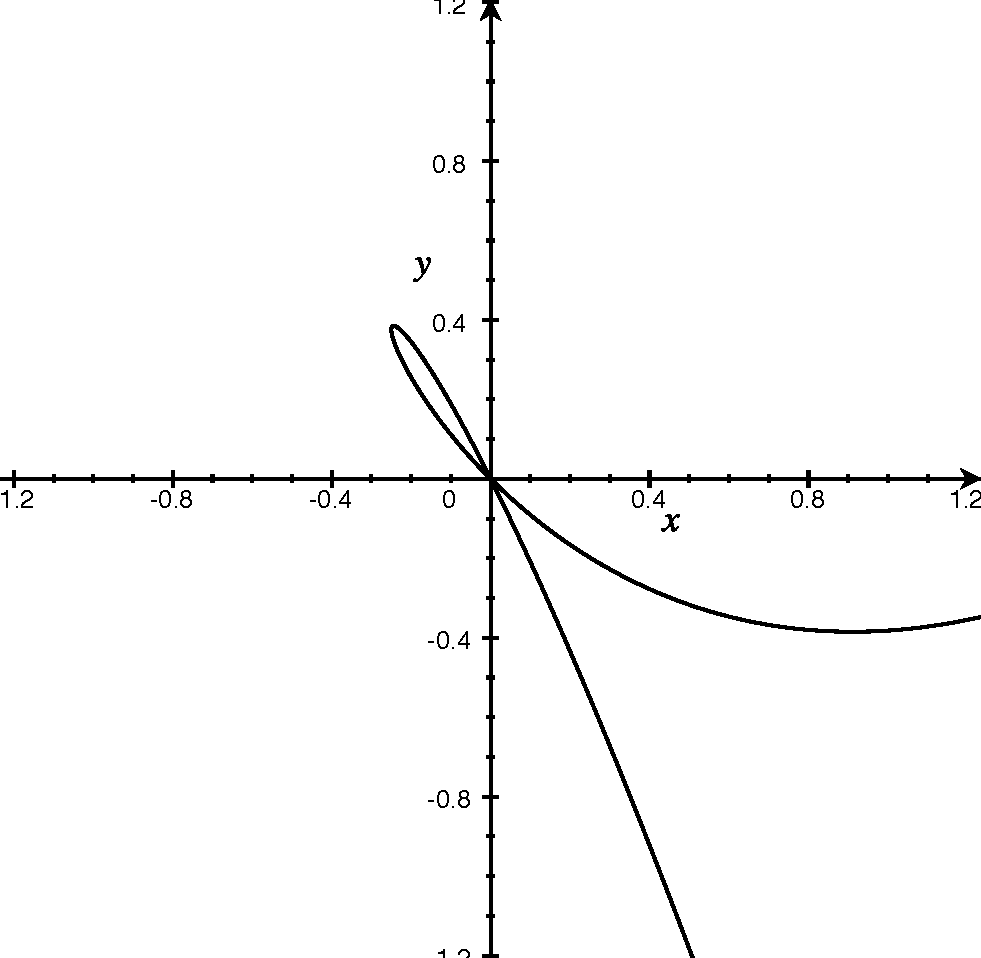
\includegraphics[width=2.5in]{graph-plus-minus.pdf}\hfill%
%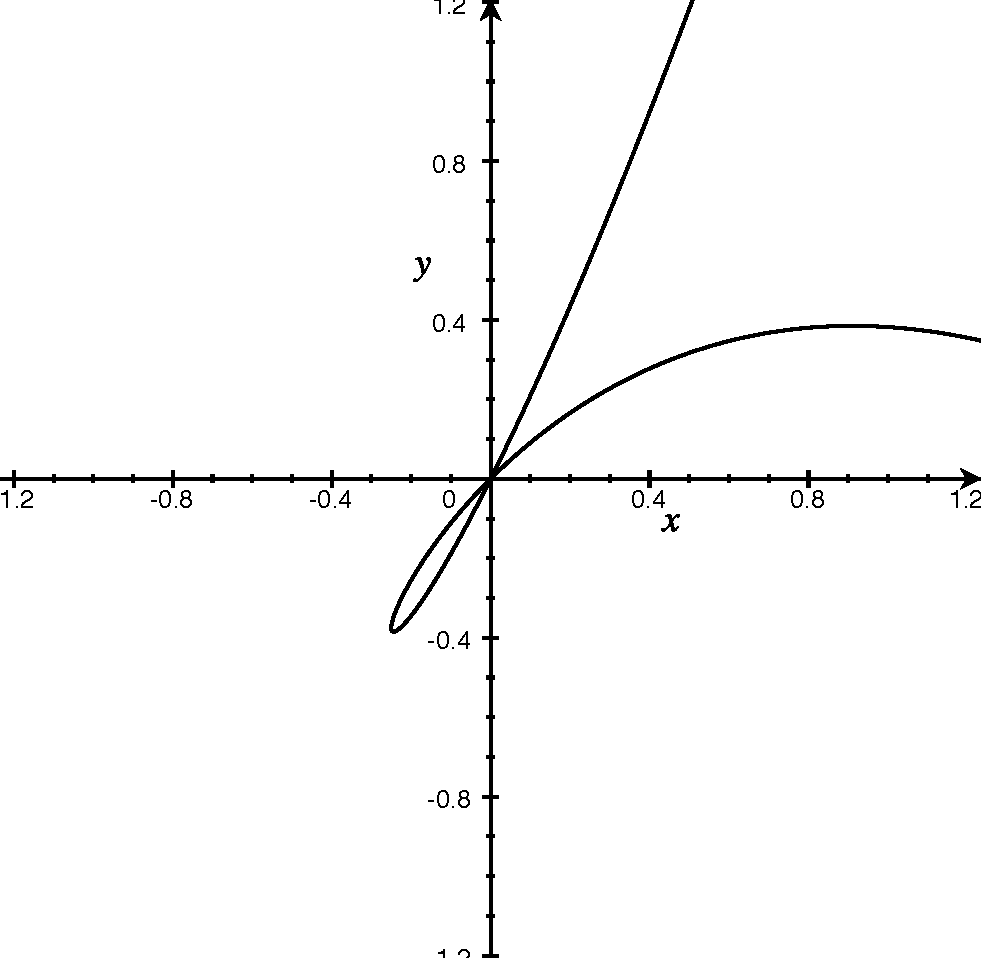
\includegraphics[width=2.5in]{graph-minus-minus.pdf}\hfill\null\\
%\vfill%
%\noindent\hfill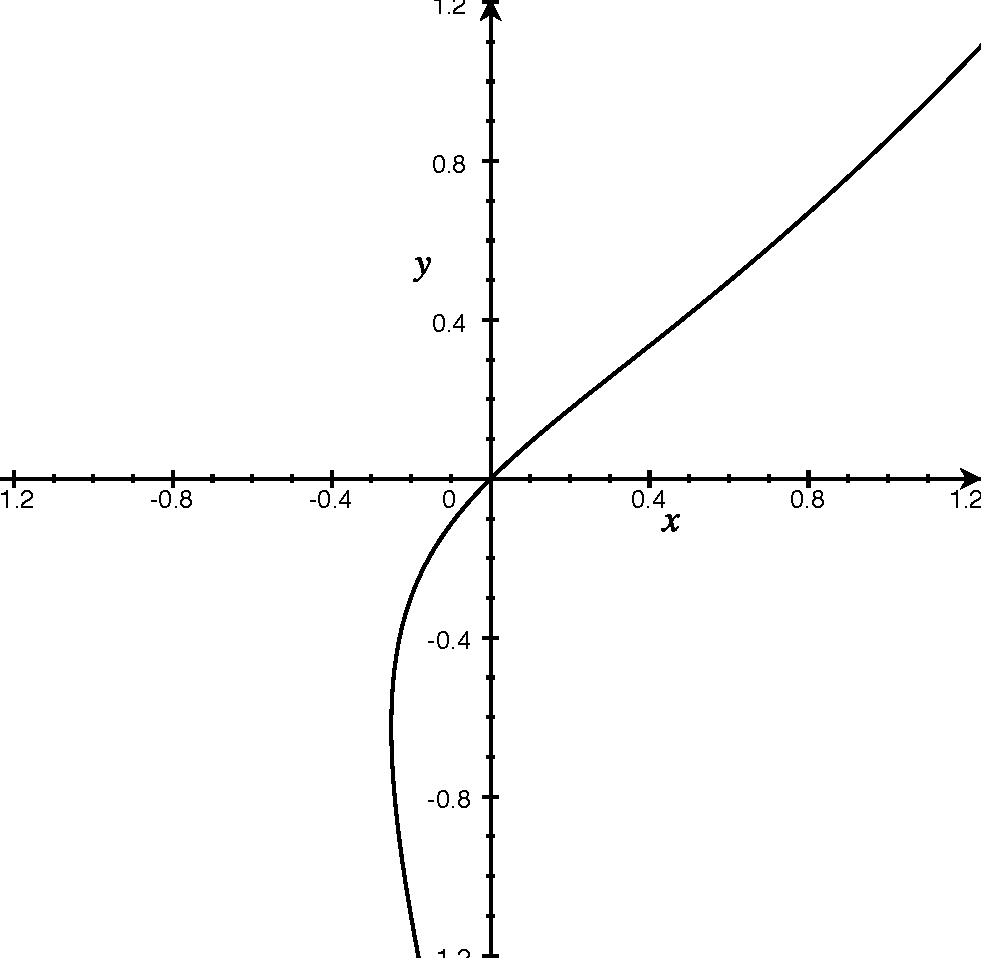
\includegraphics[width=2.5in]{graph-plus-plus.pdf}\hfill%
%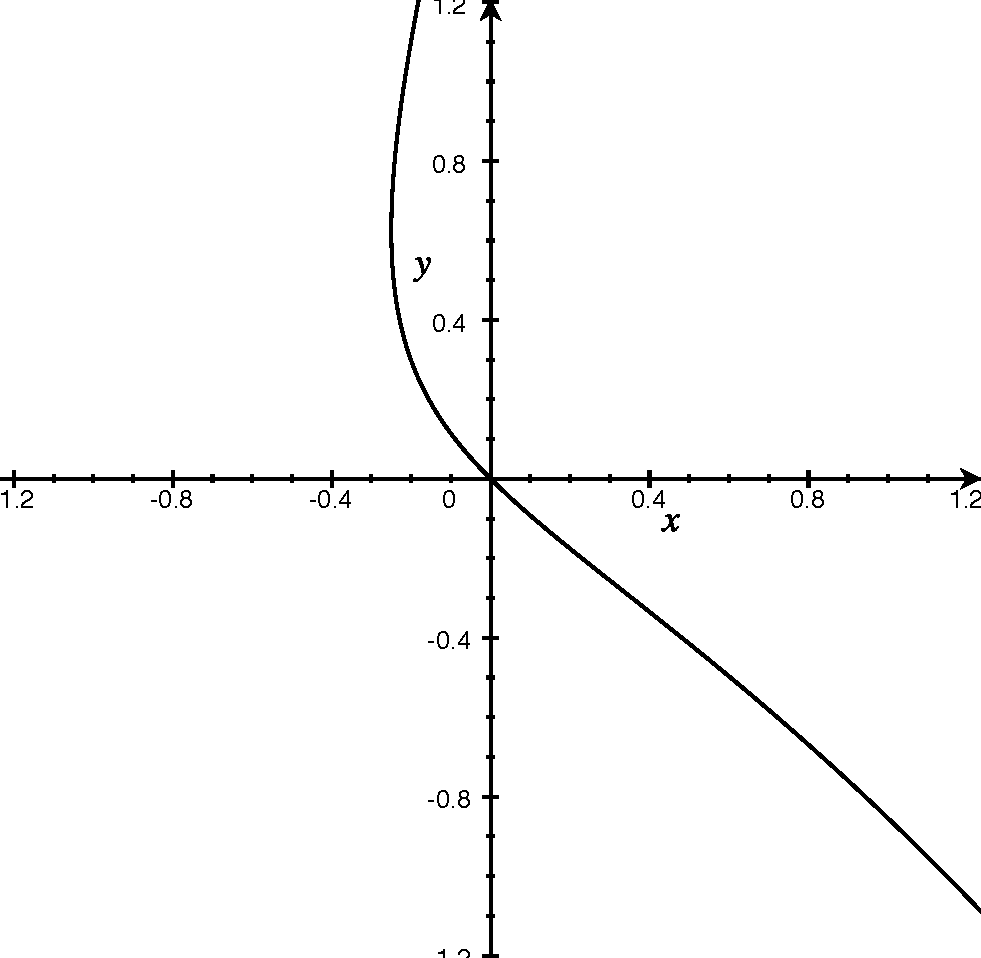
\includegraphics[width=2.5in]{graph-minus-plus.pdf}\hfill\null\\

%\vfill
\begin{solutiontext}
This problem was ill-posed; everyone received full credit.

\end{solutiontext}
\end{solution}

%%%%%%%%%%%%%%%%%%%%%%%%%%%%%%%%%%%%%%%%%%%%%%%%%%%%%%%%%%%%%%%%
%!(2) Find the slope of a tangent line to a curve given in terms of a parameter.
% Find the slope of a tangent line to a curve given in polar coordinates.
%! Differentiate and integrate vector-valued functions.
%! Caclulate unit tangent vectors to a curve.
\begin{problem}[20]
\begin{multicols}{2}
\noindent
Consider the curve given, in polar coordinates, by
$r = \theta^2$.
Find the \textbf{slope} of the tangent line to the curve when $\theta = \pi/2$.
\columnbreak
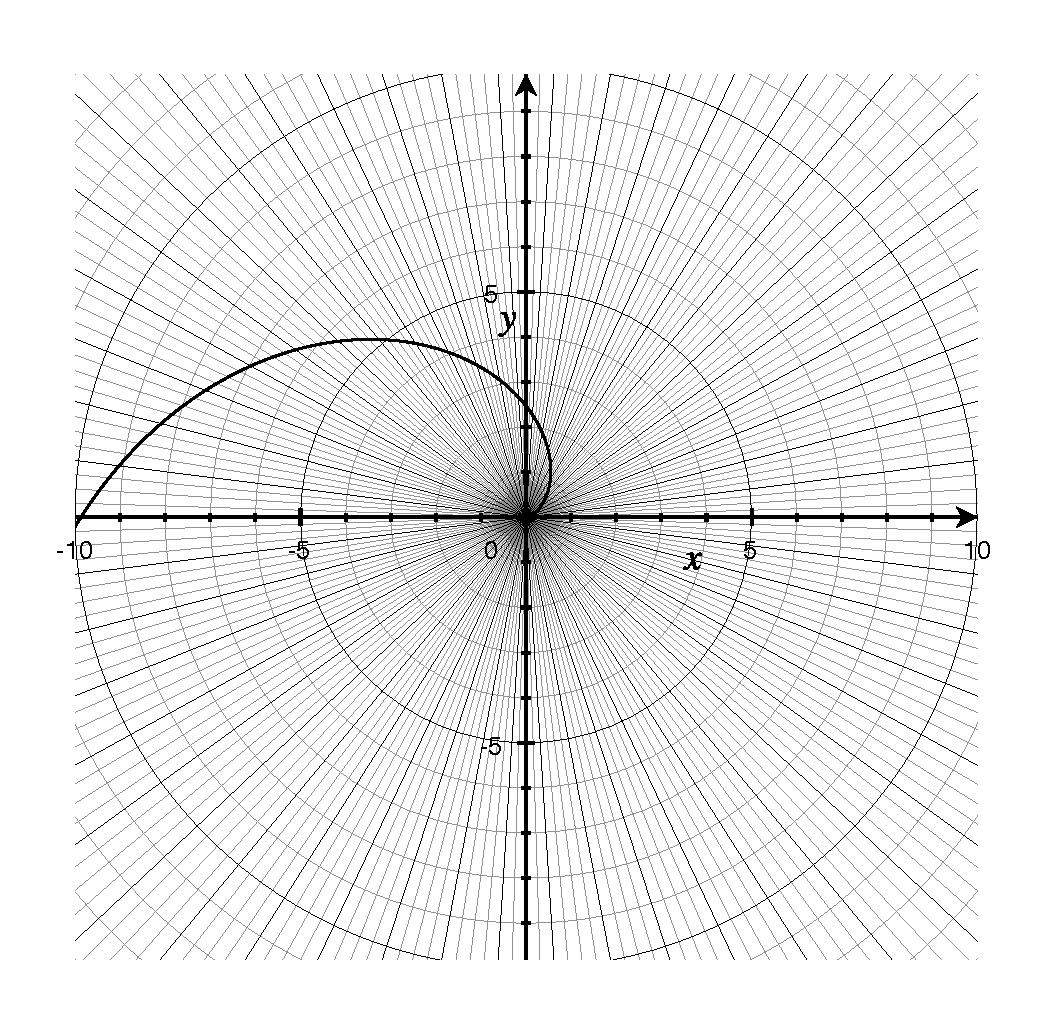
\includegraphics[width=3in]{theta-squared.pdf}
\end{multicols}
\end{problem}

\begin{solution}\begin{solutiontext}
Recall that the relationship between polar and cartesian coordinates is
\begin{eqnarray*}
x &=& r \cos \theta, \\
y &=& r \sin \theta.
\end{eqnarray*}
Using this, we convert $r = \theta^2$ into a parametric equation
\begin{eqnarray*}
x &=& \theta^2 \cos \theta, \\
y &=& \theta^2 \sin \theta.
\end{eqnarray*}
This gives the position of a point $(x,y)$ depending on $\theta$.  We differentiate to find
\begin{eqnarray*}
\frac{dx}{d\theta} &=& 2 \theta \cos \theta - \theta^2 \sin \theta, \\
\frac{dy}{d\theta} &=& 2\theta\sin\theta + \theta^2 \cos \theta.
\end{eqnarray*}
The ratio of these derivatives gives
$$
\frac{dy}{dx} = \frac{dy/d\theta}{dx/d\theta} = \frac{2 \theta \cos \theta - \theta^2 \sin \theta}{2\theta\sin\theta + \theta^2 \cos \theta}.
$$
The problem asks us to find the slope of the tangent line, $dy/dx$, when $\theta = \pi/2$.  In the graph, this looks to be roughly $-1$.  In reality, this is
\begin{eqnarray*}
\frac{dy}{dx} &=& \frac{2 \left(\pi/2\right) \cos \left(\pi/2\right) - \left(\pi/2\right)^2 \sin \left(\pi/2\right)}{2\left(\pi/2\right)\sin\left(\pi/2\right) + \left(\pi/2\right)^2 \cos \left(\pi/2\right)} \\
&=& \frac{\pi \cdot 0 - \left(\pi/2\right)^2 \cdot 1}{\pi \cdot 1 + \left(\pi/2\right)^2 \cdot 0} \\
&=& \frac{- \left(\pi/2\right)^2}{\pi} = - \frac{\pi}{4},
\end{eqnarray*}
which is a bit less than $-1$, consistent with the picture.


\end{solutiontext}\end{solution}

%%%%%%%%%%%%%%%%%%%%%%%%%%%%%%%%%%%%%%%%%%%%%%%%%%%%%%%%%%%%%%%%
%!(3) Find the angle of intersection between curves.
% Find an equation for a line through a given point and in a given direction.
\begin{problem}[25]
Consider the functions $f : \R \to \R^2$ and $g : \R \to \R^2$ given by
\begin{eqnarray*}
f(t) &=& (6t,8t) \\
g(s) &=& (3s,2s^2).
\end{eqnarray*}
The graphs intersect when $t = 1$ and $s = 2$; find the cosine of the
angle of intersection of these two curves.
\end{problem}

\begin{solution}\begin{solutiontext}
Note that $f(1) = (6,8)$ and $g(2) = (6,8)$, so they do intersect.  A common mistake was to find the angle between the vectors $f(1)$ and $g(2)$, when in fact you must find the angle between $f'(1)$ and $g'(2)$.
Since
$$
f'(t) = (6,8) \mbox{ and } g'(s) = (3,4s)
$$
we get
$$
f'(1) = (6,8) \mbox{ and } g'(2) = (3,8)
$$
The angle between the curves at the point of intersection is the angle between the vectors $(6,8)$ and $(3,8)$.
The dot product is
$$
(6,8) \cdot (3,8) = 18 + 64 = 82
$$
The length of the first vector is
$$
||f'(1)|| = \sqrt{6^2 + 8^2} = \sqrt{100} = 10.
$$
The length of the second vector is
$$
||g'(2)|| = \sqrt{3^2 + 8^2} = \sqrt{9 + 64} = \sqrt{73}.
$$
Consequently, using the geometric interpretation of the dot product,
$$
\cos \theta = \frac{f'(1) \cdot g'(2)}{||f'(1)|| \, ||g'(2)||} = \frac{82}{10 \cdot \sqrt{73}}.
$$
Some people wrote this in lowest terms, but that is, of course, not necessary.

\end{solutiontext}\end{solution}

%%%%%%%%%%%%%%%%%%%%%%%%%%%%%%%%%%%%%%%%%%%%%%%%%%%%%%%%%%%%%%%%
%!(5) Write vectors as a linear combination of other vectors.
\begin{problem}[20]
  If possible, write the vector $(8,9) \in \R^2$ as a scalar multiple
  of $(1,1)$ added to a scalar multiple of $(1,2)$.  If it is not possible, explain why.
\end{problem}

\begin{solution}\begin{solutiontext}
We want to find $\alpha, \beta \in \R$ so that
$$
(8,9) = \alpha \cdot (1,1) + \beta \cdot (1,2).
$$
In other words, we want to solve the system of equations
\begin{eqnarray*}
8 &=& \alpha \cdot 1 + \beta \cdot 1, \\
9 &=& \alpha \cdot 1 + \beta \cdot 2. \\
\end{eqnarray*}
Subtracting the second equation from the first implies $\beta = 1$.  Solving then for $\alpha$, we find $\alpha = 7$.  A quick check
$$
(8,9) = 7 \cdot (1,1) + 1 \cdot (1,2) = (7 \cdot 1 + 1 \cdot 1, 7 \cdot 1 + 1 \cdot 2)
$$
shows that this works.

\end{solutiontext}\end{solution}

%%%%%%%%%%%%%%%%%%%%%%%%%%%%%%%%%%%%%%%%%%%%%%%%%%%%%%%%%%%%%%%%
%!(6) Compute the dot product of two vectors.
%! Perform algebra with the dot product.
%! Normalize a vector (so that it has unit length).
%! Find the length of a vector.
\begin{problem}[25]
Consider two vectors in $\R^2$,
$$
v = (1,2) \mbox{ and }
w = (1,1).
$$
\begin{description}
\item[(a)] Find a unit length vector pointing in the same direction as $v$. \\
\item[(b)] Calculate $w \cdot (100 v + 1000 w)$.
\end{description}
\end{problem}

\begin{solution}\begin{solutiontext}
The lengh of $v$ is
$$
||v|| = \sqrt{1^2 + 2^2} = \sqrt{5}.
$$
To find a unit length vector, we divide $v$ by its length, to get
$$
\frac{v}{||v||} = \frac{(1,2)}{\sqrt{5}} = \left( \frac{1}{\sqrt{5}}, \frac{2}{\sqrt{5}} \right).
$$
Some people chose to rationalize the denominator (though this is not necessary).

\end{solutiontext}\end{solution}

%%%%%%%%%%%%%%%%%%%%%%%%%%%%%%%%%%%%%%%%%%%%%%%%%%%%%%%%%%%%%%%%
%!(7) Determine whether vectors are orthogonal.
%! Find the angle between two vectors.
\begin{problem}[20]
% I want cos theta = sqrt(3)/2
Compute the angle between the vectors
$(1,0,0)$ and $(\sqrt{3},0,3)$.  Are they orthogonal?
\end{problem}

\begin{solution}\begin{solutiontext}
If $\theta$ is the angle between vectors $v$ and $w$, then
$$
\cos \theta = \frac{ v \times w }{||v|| \, ||w||}.
$$
If $v = (1,0,0)$ and $w = (\sqrt{3},0,3)$, then
$$
v \times w = 1 \cdot \sqrt{3} + 0 \cdot 0 + 0 \cdot 3 = \sqrt{3}.
$$
The length of $v$ is $||v|| = 1$.  The length of $w$ is
$$
||w|| = \sqrt{(\sqrt{3})^2 + 0^2 + 3^2} = \sqrt{3 + 9} = \sqrt{12}.
$$
Therefore,
$$
\cos \theta = \frac{ v \times w }{||v|| \, ||w||} = \frac{\sqrt{3}}{1 \cdot \sqrt{12}} = \frac{1}{\sqrt{4}} = \frac{1}{2}.
$$
But the problem does not ask us to find the cosine of the angle---the
problem asks for the angle between the given vectors.  Many people
made the mistake of only determining whether or not the angles were
orthogonal without determining $\theta$.  If $\cos \theta = 1/2$, then
$\theta = \pi/3$.

Since the dot product is not zero (equivalently, since $\cos \theta$
is not zero), the given vectors are not orthogonal.

\end{solutiontext}\end{solution}

%%%%%%%%%%%%%%%%%%%%%%%%%%%%%%%%%%%%%%%%%%%%%%%%%%%%%%%%%%%%%%%%
%!(8) Compute the cross product of two vectors in $\R^3$.
% Interpret the cross product as the area of a parallelogram.
\begin{problem}[20]
Let $v = (1,1,1) \in \R^3$, and $w = (2,0,0) \in \R^3$.
\begin{description}
\item[(a)] Compute $v \times w$.
\item[(b)] Calculate the area of the parallelogram having vertices
$$
(0,0,0), \hspace{1em}
(1,1,1), \hspace{1em}
(3,1,1), \hspace{1em}
(2,0,0).
$$
\end{description}
\end{problem}

\begin{solution}\begin{solutiontext}
    To calculate the cross product in \textbf{(a)}, we rewrite $v$ as
    $i + j + k$ and $w$ as $2i$.  Then, the cross product can be computed as
\begin{eqnarray*}
v \times w &=& (i + j + k) \times (2i) \\
&=& (i \times (2i)) + (j \times (2i)) + (k \times (2i)) \\
&=& 0 + 2 (j \times i) + 2(k \times i) \\
&=& 0 - 2k + 2j,
\end{eqnarray*}
which, written as a tuple, is $(0,2,-2)$.

Next, we tackle part \textbf{(b)}.  The area of the parallelogram with vertices $0$,$v$,$w$, and $v+w$ is the length of the cross product, i.e., $||v \times w||$.  Since $v \times w = (0,2,-2)$,the area of the parallelogram is the length of $(0,2,-2)$, namely,
$$
|| v\times w || = \sqrt{0^2 + 2^2 + (-2)^2} = \sqrt{4 + 4} = \sqrt{8} = 2\sqrt{2}.
$$
Of course, $\sqrt{8}$ is a perfectly good answer.

\end{solutiontext}\end{solution}

%%%%%%%%%%%%%%%%%%%%%%%%%%%%%%%%%%%%%%%%%%%%%%%%%%%%%%%%%%%%%%%%
%!(9) Determine whether two lines intersect, are parallel, or are skew.
\begin{problem}[25]
Consider the lines
\begin{eqnarray*}
L_1 &=& \{ v \in \R^3 : v = (1,1,1) t + (0,0,0) \mbox{ for $t \in \R$ } \}, \\
L_2 &=& \{ v \in \R^3 : v = (1,1,2) t + (2,2,0) \mbox{ for $t \in \R$ } \}.
\end{eqnarray*}
Do $L_1$ and $L_2$ intersect? If they intersect, find the point of
intersection; if not, determine whether $L_1$ and $L_2$ are parallel or skew.
\end{problem}

\begin{solution}\begin{solutiontext}
They do intersect.  We search for $t,s\in \R$ so that
$$
(1,1,1) t + (0,0,0) = (1,1,2) s + (2,2,0).
$$
Next, replace this single vector equation with three equations,
\begin{eqnarray*}
1 \cdot t + 0 &=& 1 \cdot s + 2, \\
1 \cdot t + 0 &=& 1 \cdot s + 2, \\
1 \cdot t + 0 &=& 2 \cdot s + 0. \\
\end{eqnarray*}
Subtracting the third equation from the second gives
$0 = s - 2$, so $s = 2$.  Solving for $t$ then, $t = 4$.

The problem asks us to find the point where these lines intersect (and
a common mistake was forgetting to do this).  Substituting $t = 4$
into the first equation, we find that the point of intersection is
$$
(4,4,4) = (1,1,1) \cdot 4 + (0,0,0).
$$

\end{solutiontext}\end{solution}

%%%%%%%%%%%%%%%%%%%%%%%%%%%%%%%%%%%%%%%%%%%%%%%%%%%%%%%%%%%%%%%%
% Find an equation for a plane through a given point and with a given normal vector
%(10) Find the point of intersection between a line and a plane.
\begin{problem}[25]
  Suppose $P$ is a plane containing the point $(1,1,1)$ and having
  normal vector $(4,5,-6)$.
\begin{description}
\item[(a)] Write down an equation for the plane $P$.
\item[(b)] Find the intersection of $P$ with the line
$$
L = \{ v \in \R^3 : v = t \cdot (1,1,1) + (0,0,0) \mbox{ for $t \in \R$} \},
$$
or, if they do not intersect, prove it.
\end{description}
\end{problem}

\begin{solution}\begin{solutiontext}
For part \textbf{(a)}, you should write down the formula for a plane through a point $b$ and with normal vector $n$, namely,
$$
P = \{ v \in \R^3 : (v - b) \cdot n = 0 \}.
$$
So in this case,
$$
P = \{ v \in \R^3 : \left(v - (1,1,1) \right) \cdot (4,5,-6) = 0 \}.
$$
Of course, there are other ways of writing down an equation for a plane, and I gave credit for any of them.  For instance, you might rewrite this as
$$
\left((x,y,z) - (1,1,1) \right) \cdot (4,5,-6) = 0
$$
and then expand out to get
$$
4x + 5y - 6z = 3.
$$
I meant part \textbf{(b)} to be really easy: the line $L$ includes the point $(1,1,1)$, and the plane $P$ also contains the point $(1,1,1)$, so they intersect at that point.  You could have written down a system of linear equations and solved it, too, but you don't need to if you can see the solution right away.

\end{solutiontext}\end{solution}

%%%%%%%%%%%%%%%%%%%%%%%%%%%%%%%%%%%%%%%%%%%%%%%%%%%%%%%%%%%%%%%%
% bonus true/false questions
\begin{problem}[0]
  The following ten questions are for extra credit.  \textbf{Circle} the best
    answer.

\begin{description}
\vfill
\item[\FalseChoice] There are four vectors $v_1,v_2,v_3,v_4 \in \R^3$ so that $v_i$ and $v_j$ are orthogonal for $i \neq j$.  \begin{solutiontext}\textit{I meant this problem to ask for \textit{nonzero} vectors; as stated, it is true, if you use the zero vector.  I gave credit for either answer.}
\end{solutiontext}
\vfill
\item[\TrueChoice] If $v_1, v_2 \in \R^3$, then $v_1 \times v_2$ is orthogonal to both $v_1$ and $v_2$.  \begin{solutiontext}\textit{This is a property of the cross product.}\end{solutiontext}
\vfill
\item[\TrueChoice] There are two lines in $\R^3$ which do not intersect and are not parallel.  \begin{solutiontext}\textit{This is the definition of \textit{skew} lines.}\end{solutiontext}
\vfill
\item[\FalseChoice] If $f(t) = (t,t^2,t^3)$, then
  $\displaystyle\frac{df}{dt} = (1,2,3)$ when $t = 0$.  \begin{solutiontext}\textit{This is actually the derivative evaluated at $t=1$ not $t=0$.}\end{solutiontext}
\vfill
\item[\TrueChoice] Given a vector $v \in \R^3$, it is possible to find six unit vectors in $\R^3$ which are each orthogonal to $v$.  \begin{solutiontext}\textit{You can find infinitely many vectors perpendicular to a given vector}\end{solutiontext}
\vfill
\item[\FalseChoice] If $v,w,u$ are vectors in $\R^3$, then $((v \cdot u) \cdot w) \times v$ is zero.  \begin{solutiontext}\textit{}\end{solutiontext}
\vfill
\item[\FalseChoice] Suppose $v \in \R^2$ is a unit vector; there does not exist a vector $w \in \R^2$ so that $v \cdot w = 10^{10}$.  \begin{solutiontext}\textit{There does exist such a vector---you can choose $w = 10^{10} \cdot v$.}\end{solutiontext}
\vfill
\item[\TrueChoice] Given a line $L$ in $\R^3$, it is possible to find
  two planes $P_1$ and $P_2$ so that $P_1$ and $P_2$ do not intersect
  $L$, but $P_1$ intersects $P_2$ in a line.  \begin{solutiontext}\textit{Choose two planes that are not parallel, but which do not contain the line $L$.}\end{solutiontext}
\vfill
\item[\TrueChoice] For all vectors $v, w \in \R^3$, it is the case that
$$
\left((4w) \times (3v)\right) \cdot (5w) = \left((3v) \times (4w)\right) \cdot (4w).$$\begin{solutiontext}\textit{In fact, both sides are zero.}\end{solutiontext}
\vfill
\item[\TrueChoice] For vectors $v, w \in \R^4$, it is always the case that
$$
(v + w) \cdot (v + w) = ||v||^2 + ||w||^2 + 2 \cdot (v \cdot w).
$$\begin{solutiontext}\textit{You can prove this by using the distributive property.}\end{solutiontext}
\vfill
\null
\end{description}

\end{problem}

%\ifthenelse{\equal{\HasSolutions}{true}}{}{%
%\pagebreak%
%\section*{Extra Paper}%
%\pagebreak%
%\null%
%\pagebreak%
%\null%
%\pagebreak%
%\null%
%\pagebreak%
%\null%
%}

%%%%%%%%%%%%%%%%%%%%%%%%%%%%%%%%%%%%%%%%%%%%%%%%%%%%%%%%%%%%%%%%
\addtocontents{toc}{\textbf{Total} \protect& \protect& /\arabic{totalpoints}}

\end{document}
